\chapter{Kompleksitas Algoritma}\label{ch:modul6}


\section{Pengenalan Kompleksitas Algoritma}
Waktu yang diperlukan bagi \textit{Insertion Sort} untuk menyelesaikan proses pengurutannya tergantung pada jumlah masukan. Dengan kata lain, semakin besar jumlah masukan, semakin lama waktu yang diperlukan. Untuk dua masukan dengan jumlah yang sama, \textit{Insertion Sort} bisa memakan waktu yang berbeda tergantung dari seberapa terurutnya mereka. Dari sini, kita bisa mengambil kesimpulan bahwa, waktu yang diperlukan berkembang sesuai dengan ukuran dari masukan.

Besar masukan sebuah algoritma sangat tergantung terhadap permasalahan yang sedang dihadapi. Sebagai contohnya, jika berbicara mengenai permasalahan pengurutan maka besar masukan berupa berapa banyak bilangan dalam sebuah \textit{array} (\textit{array size}). Untuk permasalahan lain seperti misalnya permasalahan pencarian rute terpendek dimana masukannya adalah berupa \textit{graph} (akan dijelaskan di mata kuliah struktur data), maka yang menjadi besar masukannya adalah jumlah \textit{vertice} dan \textit{edge} dari \textit{graph} tersebut. 

\section{Analisis algoritma}
Untuk mengetahui seberapa effisien sebuah algoritma bisa dilakukan setelah menganalisis kompleksitas dari algoritma tersebut. Melakukan analisis algoritma berarti memprediksi berapa sumber daya (misalnya berapa lama waktu eksekusi atau berapa besar memori yang dibutuhkan) yang dibutuhkan oleh sebuah program ketika mengeksekusi algoritma tersebut. Pada umumnya, fokus analisis ditujukan pada waktu eksekusi dari algoritma tersebut walaupun tidak tertutup kemungkinan untuk menganalisi faktor lain.

Untuk mempermudah proses analisis, kita akan mengasumsikan bahwa algoritma kita akan berjalan di sebuah komputer dengan prossesor tunggal dan \textit{random-access machine} (RAM). Model RAM yang kita adopsi adalah model yang menjalankan algoritma secara baris per baris instruksi tanpa ada proses parallel. 

Instruksi yang diperbolehkan untuk dijalankan pada umumnya adalah instruksi penjumlahan `+', pengurangan `-', perkalian `*', pembagian `/', modulus `\%', pembulatan atas `$\left\lceil\  \right\rceil$', dan pembulatan bawah `$\left\lfloor\ \right\rfloor$', penyimpanan/pengeluaran/duplikat data ke variabel (mis: $a = 5$ dan $a = b$), dan kontrol (IF, FOR, WHILE, RETURN dan sebagainya). Semua dari instruksi tersebut menggunakan waktu secara konstan (artinya memiliki nilai yang sama apapun kondisinya, kecuali disebutkan secara eksplisit).

Untuk setiap analisis, ada tiga jenis kasus yang mungkin terjadi, yaitu: kasus terbaik, kasus terburuk dan kasus rata-rata. Dalam pengurutan, kasus terbaik adalah ketika kita hendak mengurutkan rangkaian bilangan yang sudah terurut. Sedangkan kasus terburuk adalah ketika kita hendak mengurutkan rangkaian bilang yang terurut terbalik. Untuk kasus-kasus rangkaian bilang acak lainnya, kita gunakan kasus rata-rata.

\section{Contoh Kasus: Analisis Faktorial Iteratif}
Berikut adalah hasil analisis dari Faktorial Iteratif.
\begin{figure}%
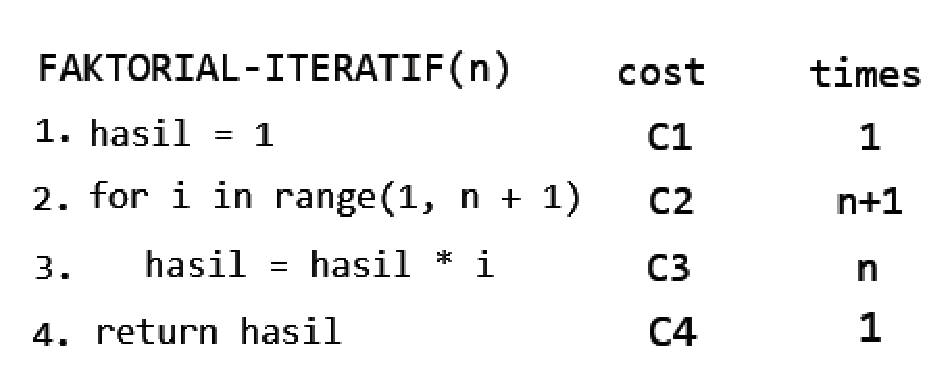
\includegraphics[scale=0.5]{fig/faktorialAnalysis}%
\caption{Analisis Faktorial}%
\label{fig:faktorialAnalysis}%
\end{figure}

\FloatBarrier
Untuk mempermudah perhitungan, biasanya setiap langkah dianggap menghabiskan waktu yang konstan yaitu konstanta $c_i$ dimana $i$ menandakan baris keberapa dari \textit{pseudocode} algoritma tersebut. Nilai dari $c_i$ sendiri tidaklah penting, yang penting adalah berapa kali konstanta $c_i$ itu dieksekusi. Dari Gambar \ref{fig:faktorialAnalysis}, setiap langkah (baris) memiliki biaya (\textit{cost}) eksekusi. 
Biaya eksekusi tersebut dilambangkan dengan besarnya konstanta $c_i$ yang dikalikan banyaknya konstanta tersebut dieksekusi yaitu $n$, dengan kata lain lamanya waktu yang dibutuhkan untuk mengeksekusi setiap langkah adalah $c_{i}\times{}n$ atau disingkat $c_{i}n$

\FloatBarrier
Penjelasan lebih detil dari Gambar \ref{fig:faktorialAnalysis} adalah sebagai berikut.
\begin{enumerate}
	\item Baris 1: Memiliki biaya sebesar $c_1$ dimana biaya tersebut akan diulang sebesar $1$ kali.  
	\item Baris 2: Memiliki biaya sebesar $c_2$ dimana biaya tersebut akan diulang sebesar $n+1$ kali. Pengulangan sebesar $n+1$ kali dikarenakan adanya sebuah looping ``\textbf{for} $i=1$ \textbf{to} $n$''. Looping \textbf{for} akan dieksekusi oleh komputer sebanyak $n+1$ kali. Untuk mempermudah perhitungan maka kita misalkan $n$ bernilai 5, maka baris 2 akan diulang sebanyak 6 kali (1,2,3,4 dan 5 bernilai $True$ dan 1 kali terakhir bernilai $False$) atau $n$+1 kali.
	\item Baris 3: Memiliki biaya $c_{3}$. Ketiga baris tersebut masing-masing diulang sebanyak $n$ kali. Kenapa $n$ kali? Karena semua baris di dalam \textit{looping} \textbf{for} hanya diulang untuk setiap \textbf{for} yang bernilai $True$.
	\item Baris 4: Memiliki biaya 0 karena baris tersebut tidak benar-benar dijalankan oleh program.
\end{enumerate}

Total waktu eksekusi dari Algoritma Faktorial Iteratif dilambangkan dengan $T(n)$ dimana:
\begin{equation}
\label{eq:eksekusiFaktorial1}
T(n) = c_{1} + c_{2}(n+1) + c_3{n} = (c_{2}+c_{3})n + (c_{1}+c_{2}+1)
\end{equation} 

Persamaan \ref{eq:eksekusiFaktorial1} bisa disederhanakan menjadi $T(n)$ = $an$ + $b$. 


Dari persamaan \ref{eq:eksekusiFaktorial1} yaitu $an$ + $b$, terdapat dua konstan ($a$, dan $b$) yang besarnya tergantung pada $c_i$. Untuk membuat lebih sederhana, kita bisa membuat abstraksi yang lebih sederhana yaitu dengan hanya memperhatikan laju pertumbuhan fungsi (\textit{order of growth}). Untuk itu kita cukup hanya perlu memperhatikan order tertinggi dari fungsi yaitu $an$ karena order yang lebih rendah lajut pertumbuhannya tidak begitu signifikan untuk nilai $n$ yang besar. Untuk itu kita tulis bahwa \textit{insertion sort} memiliki waktu eksekusi $\theta(n)$.

\section{Contoh Kasus: Analisis \textit{Bubble Sort}}

Berikut adalah \textit{pseudocode} dari Bubble Sort:

\begin{algorithm}
	\caption{BUBBLE-SORT($A$)}
	\label{algo:bubble}
	\begin{algorithmic}[1]
	\FOR {$i = 1$ \TO $A.length-1$}
		\FOR {$j = i+1$ \TO $A.length$}
			\IF {$A[i] \leq A[j]$}
			\STATE $temp = A[i]$
			\STATE $A[i] = A[j]$
			\STATE $A[j] = temp$
			\ENDIF
		\ENDFOR
	\ENDFOR
	\end{algorithmic}
\end{algorithm}

Sebelum menganalisis Algoritma \ref{algo:bubble} ada dua hal penting yang harus dipahami terlebih dahulu: besar masukan (\textit{input size}) dan waktu eksekusi (\textit{running time}). 
\begin{figure}[htbp]%
	\includegraphics[scale=0.6]{fig/BubbleAnalysis}%
	\caption{Analisis \textit{Bubble Sort}}%
	\label{fig:analisisBubbleSort}%
\end{figure}

\FloatBarrier

Algoritma \textit{Insertion Sort} bisa dilihat di Algoritma \ref{algo:insertion}. 
\begin{algorithm}[H]
	\caption{\textit{INSERTION-SORT(A)}}
	\label{algo:insertion}
	\begin{algorithmic}[1]
	\FOR {$j = 2$ to $A.length$}
		\STATE $key = A[j]$
		\STATE $i = j - 1$
		\WHILE {$i > 0$ and $A[i] > key$}
			\STATE $A[i+1] = A[i]$
			\STATE $i = i - 1$
		\ENDWHILE
		\STATE $A[i+1] = key$
	\ENDFOR
	\end{algorithmic}
\end{algorithm} 

Penjelasan lebih detil dari Gambar \ref{fig:analisisInsertionSort} adalah sebagai berikut.
\begin{enumerate}
	\item Baris 1: Memiliki biaya sebesar $c_1$ dimana biaya tersebut akan diulang sebesar $n$ kali. Pengulangan sebesar $n$ kali dikarenakan adanya sebuah loop	ing ``\textbf{for} $i=1$ \textbf{to} $A.length-1$''. Looping \textbf{for} akan dieksekusi oleh komputer sebanyak $(A.length-1)+1$ kali.
	\item Baris 2 \& 7: Baris ini diulang sebanyak $\sum\limits_{i=2}^n i$ kali. 
	\item Baris 3 \& 6: Baris ini diulang sebanyak $\sum\limits_{i=1}^{n-1} i$ kali.
	\item Baris 4 - 6: Baris ini diulang sebanyak $\sum\limits_{i=1}^{n-1} t_{i}$ kali.
\end{enumerate} 

Total waktu eksekusi dari Algoritma \ref{algo:insertion} dilambangkan dengan $T(n)$ dimana:
\begin{equation}
\label{eq:eksekusiBubble1}
T(n) = c_{1}n + c_{2}\sum\limits_{i=2}^n i + c_{3}\sum\limits_{i=1}^{n-1} i + (c_{4}+c_{5}+c_{6})\sum\limits_{i=1}^{n-1} t_{i} 
\end{equation} 

Seandainya semua bilangan sudah terurut maka baris ke 4, 5 dan 6 dari Algoritma \ref{algo:insertion} tidak perlu dijalankan lagi karena perintah di baris ke 5 akan selalu menghasilkan $False$. Dengan kata lain nilai dari $t_{i}$ bernilai 0 karena tidak pernah dijalankan. Maka Persamaan \ref{eq:eksekusiBubble1} akan menjadi sebagai berikut.
\begin{eqnarray}
T(n) & = & c_{1}n + c_2((n-1)(n-2))/2+c_3((n-1)n)/2
\label{eq:eksekusiBubble2}
\end{eqnarray}

Persamaan \ref{eq:eksekusiBubble2} merupakan apa yang biasa disebut sebagai \textit{best case} atau kasus terbaik. Jika persamaan tersebut disederhanakan maka bisa ditulis sebagai $an^2+bn+c$. 

Untuk kasus terburuk (\textit{worst case}) akan terjadi jika \textit{array} angka yang akan diurut disusun secara terbalik semua (misalnya mengurut bilangan $\left\{5,4,3,2,1\right\}$ menjadi $\left\{1,2,3,4,5\right\}$). Untuk kasus tersebut, berarti kita harus mencocokkan setiap angka di \textit{inner loop}, atau dengan kata lain nilai dari $t_{i}$ adalah sama dengan nilai dari $i$. 

\begin{eqnarray}
T(n) & = & c_{1}n + c_2((n-1)(n-2))/2+(c_3+c_4+c_5+c_6)(((n-1)n)/2)
\label{eq:eksekusiBubble3}
\end{eqnarray}

Persamaan \ref{eq:eksekusiBubble3} bisa disederhanakan menjadi $an^2+bn+c$ atau yang disebut juga dengan fungsi kuadratic akan $n$. 

Baik \textit{Best Case} dan \textit{Worst Case} sama-sama memiliki nilai $\theta(n^2)$.

\section{Contoh Kasus: Analisis \textit{Insertion Sort}}
Berikut adalah analisis dari Algoritma \ref{algo:insertion}.
\begin{figure}[htbp]%
	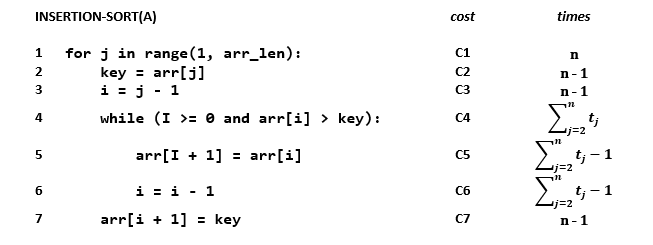
\includegraphics[scale=0.7]{fig/InsertionSortAnalysis}%
	\caption{Analisis \textit{Insertion Sort}}%
	\label{fig:analisisInsertionSort}%
\end{figure}

\FloatBarrier
Penjelasan lebih detil dari Gambar \ref{fig:analisisInsertionSort} adalah sebagai berikut.
\begin{enumerate}
	\item Baris 1: Memiliki biaya sebesar $c_1$ dimana biaya tersebut akan diulang sebesar $n$ kali. Pengulangan sebesar $n$ kali dikarenakan adanya sebuah loop	ing ``\textbf{for} $j=2$ \textbf{to} $A.length$''. Looping \textbf{for} akan dieksekusi oleh komputer sebanyak $A.length+1$ kali. Untuk mempermudah perhitungan maka kita lambangkan $A.length+1$ sebagai $n$. Sebagai contohnya, jika $A.length$ bernilai 5, maka baris 1 akan diulang sebanyak 6 kali (1,2,3,4 dan 5 bernilai $True$ dan 1 kali terakhir bernilai $False$) atau dengan kata lain $n$ bernilai 6.
	\item Baris 2 -- 4: Memiliki biaya masing-masing $c_{2}$, 0, dan $c_{4}$. Baris ke 3 bernilai 0 dikarenakan merupakan komentar yang tidak memakan sumber daya komputer. Ketiga baris tersebut masing-masing diulang sebanyak $n-1$ kali. Kenapa $n-1$ kali? Karena semua baris di dalam \textit{looping} \textbf{for} hanya diulang untuk setiap \textbf{for} yang bernilai $True$.
	\item Baris 5: Baris ini diulang sebanyak $\sum\limits_{j=2}^n t_{j}$ kali. Di baris ini ada dua buah \textit{looping}: \textit{outer loop} -- \textbf{for} dan \textit{inner loop} -- \textbf{while}. Untuk \textit{inner loop} dilambangkan dengan $t_{j}$. $t_{j}$ melambangkan jumlah \textit{looping inner loop}. Ketika \textit{inner loop} dan \textit{outer loop} digabungkan maka menjadi $\sum\limits_{j=2}^n t_{j}$.  
\end{enumerate}                                       
                                     
Total waktu eksekusi dari Algoritma \ref{algo:insertion} dilambangkan dengan $T(n)$ dimana:
\begin{equation}
\label{eq:eksekusiInsertion1}
T(n) = c_{1}n + c_{2}(n-1) + c_{4}(n-1) + c_{5}\sum\limits_{j=2}^n t_{j} + c_{6}\sum\limits_{j=2}^n (t_{j}-1) + c_{7}\sum\limits_{j=2}^n (t_{j}-1) + c_{8}(n-1) 
\end{equation} 

Dari Persamaan \ref{eq:eksekusiInsertion1}, kita bisa menghitung total waktu eksekusi ($T(n)$) yang bergantung kepada variabel $n$ atau banyaknya bilangan masukan. Semakin banyak bilangan masukan maka $T(n)$ akan semakin tinggi dan sebaliknya. Akan tetapi, $T(n)$ tidak hanya bergantung pada banyaknya bilangan masukan, tetapi bergantung juga kepada susunan bilangan tersebut. Bagaimana jika \textit{array} bilangan tersebut sudah terurut? Bukankah waktu yang dibutuhkan akan lebih sedikit dibandingkan jika semua bilangan tersebut terbalik urutannya?

Seandainya semua bilangan sudah terurut maka baris ke 6 dan baris ke 7 dari Algoritma \ref{algo:insertion} tidak perlu dijalankan lagi karena perintah di baris ke 5 akan selalu menghasilkan $False$. Dengan kata lain nilai dari $t_{j}$ akan selalu konstan yaitu 1. Maka Persamaan \ref{eq:eksekusiInsertion1} akan menjadi sebagai berikut.
\begin{eqnarray}
T(n) & = & c_{1}n + c_2(n-1)+c_4(n-1)+c_5(n-1)+c_8(n-1)
\nonumber \\
 & = & (c_1+c_2+c_4+c_5+c_8)n-(c_2+c_4+c_5+c_8)
\label{eq:totalEksekusi3}
\end{eqnarray}

Persamaan \ref{eq:eksekusiInsertion1} merupakan apa yang biasa disebut sebagai \textit{best case} atau kasus terbaik. Jika persamaan tersebut disederhanakan maka bisa ditulis sebagai $an+b$ atau yang biasa disebut sebagai fungsi linear akan $n$. 

Untuk kasus terburuk (\textit{worst case}) akan terjadi jika \textit{array} angka yang akan diurut disusun secara terbalik semua (misalnya mengurut bilangan $\left\{5,4,3,2,1\right\}$ menjadi $\left\{1,2,3,4,5\right\}$). Untuk kasus tersebut, berarti kita harus mencocokkan setiap angka di \textit{inner loop}, atau dengan kata lain nilai dari $t_{j}$ adalah sama dengan nilai dari $j$ yang berasal dari \textit{outer loop}. 

\begin{eqnarray}
T(n) & = & c_1n + c_2(n-1) + c_4(n-1) + c_5(\frac{n(n+1)}{2}-1) + c_6(\frac{n(n-1)}{2})   \nonumber \\ 
& & + c_7(\frac{n(n-1)}{2})+c_8(n-1) 
\nonumber \\ 
 & = & (\frac{c_5}{2}+\frac{c_6}{2}+\frac{c_7}{2})n^2+(c_1+c_2+c_4+\frac{c_5}{2}-\frac{c_6}{2}-\frac{c_7}{2}+c_8)n \nonumber\\
& & -(c_2+c_4+c_5+c8)
\label{eq:eksekusiInsertion2}
\end{eqnarray}

Persamaan \ref{eq:eksekusiInsertion2} bisa disederhanakan menjadi $an^2+bn+c$ atau yang disebut juga dengan fungsi kuadratic akan $n$. 

Dari persamaan \ref{eq:eksekusiInsertion2} yaitu $an^2+bn+c$, terdapat tiga konstan ($a$, $b$, dan $c$) yang besarnya tergantung pada $c_i$. Untuk membuat lebih sederhana, kita bisa membuat abstraksi yang lebih sederhana yaitu dengan hanya memperhatikan laju pertumbuhan fungsi (\textit{order of growth}). Untuk itu kita cukup hanya perlu memperhatikan order tertinggi dari fungsi yaitu $an^2$ karena order yang lebih rendah lajut pertumbuhannya tidak begitu signifikan untuk nilai $n$ yang besar. Untuk itu kita tulis bahwa \textit{insertion sort} memiliki \textit{worst case} $\theta(n^2)$.
